\documentclass[12pt]{article}

\usepackage{graphicx}
\usepackage[doublespacing]{setspace}
\usepackage{textcomp}
\usepackage{amsmath,bm}
\usepackage{amssymb}
\usepackage{fancyhdr}
\usepackage{lastpage}
\usepackage{float}
\usepackage{array}
\usepackage{indentfirst}
\usepackage{titletoc}
\usepackage{setspace,geometry}
\titlecontents{chapter}[0pt]{\addvspace{2pt}\filright}
              {\contentspush{\thecontentslabel\ }}
              {}{\titlerule*[8pt]{.}\contentspage}
\setlength{\parindent}{2em}
\pagestyle{fancy}
\title{}
\lhead{Team \# 85397}
\rhead{Page \thepage{} of \pageref{LastPage}}
\cfoot{}
\title{TITLE}
\author{YuHaiyang, HuangLingjia and WangZhongnan}
\date{}
\begin{document}
\maketitle
\setlength{\baselineskip}{15pt}
\begin{center}

\end{center}

\noindent \textbf{\large Abstract}

\noindent The article analyzed and predicted the condition of energy usage in AZ, CA, NM, TX and put some suggestions on rational utilization of resources and environment protection. \ \ {Part \uppercase\expandafter{\romannumeral1}.} It used linear regression model to get the information about total amount and variation tendency of traditional energy and new energy. Secondly, considering $\mathrm{CO_{2}}$, $\mathrm{SO_{2}}$, $\mathrm{NO}_{x}$, $\mathrm{PM_{2.5}}$ and renewable as the indexes of the "best", using TOPSIS method ,it concluded that CA is the "best". Next, it used linear regression prediction and polynomial curve fitting to predict the probability values and the prediction intervals from 2025 to 2050.{\ \ Part
\uppercase\expandafter{\romannumeral2}}.It take the lower prediction interval limit and the upper prediction interval limit as the goals for each state.Then,on the aspect of population, geography and industry; reduction pollution; and price of energy, it put forward 3 proposals to achieve the goals.\ \
{\ \ Part \uppercase\expandafter{\romannumeral3}.} It offered an memo which summarized all the results of analysis and predictions to governors.


\noindent \textbf{ Keywords:} Polynomial Curve Fitting \ \ \ Regression Analysis Prediction\  TOPSIS Method\ \ \ Linear Regression

\newpage
\tableofcontents
\newpage
\section{\leftline{Introduction}}

\noindent Interstate compacts represent an opportunity for multi-state cooperation, reinforcing state sovereignty and avoiding federal intervention. Compacts enable the states in their sovereign capacity to act jointly and collectively, generally outside the confines of the federal legislative or regulatory process while respecting the view of Congress on the appropriateness of joint action. [1] Thus, states sometimes have interstate compacts for their own development. The Southern States Energy Board (SSEB), a multi-state regional organization, was committed to promote economic development and quality of life in the southern United States through innovations in energy and the environment. The California (CA) , Arizona (AZ), New Mexico (NM) and Texas (TX) four states were once members of this organization. [2]

\section{\leftline{Assumptions}}

1. Divide all types of energy into primary energy and secondary energy. We don't take secondary energy into consideration and regard all the amount of primary energy as total consumption (including the primary energy which convert to heat or secondary energy)

2. Define nuclear energy, hydrogen, wood and waste, biomass, geothermal energy, wind energy, photovoltaic and solar thermal energy are cleaner or renewable energy;natural gas, coal and petroleum aren't cleaner and renewable.

3.All the primary energy which is cleaner and renewable energy is consumed in the
local state. In other words, the production of primary energy is equal to the total consumption
of it.

\section{\leftline{Notations}}
\newpage
\begin{table}[!h]\centering\small
\begin{tabular}{|c|l| }
\hline
 notation&description\\
 \hline
$x_{A}$&traditional energy consumption in AZ\\
\hline
$y_{A}$&new energy consumption in AZ\\
\hline
$x_{C}$&traditional energy consumption in CA\\
\hline
$y_{C}$&new energy consumption in CA\\
\hline
$x_{N}$&traditional energy consumption in NM\\
\hline
$y_{N}$&new energy consumption in NM\\
\hline
$x_{T}$&traditional energy consumption in TX\\
\hline
$y_{T}$&new energy consumption in TX\\
\hline
$t$&years(from 1960 to 2050)\\
\hline
\end{tabular}
\end{table}


\section{\leftline{Part \uppercase\expandafter{\romannumeral1}}}

\subsection{Part \uppercase\expandafter{\romannumeral1}  A}



In order to get the energy profiles of each state, we analyze TEPRB(The total energy production), TETGR(The total energy consumed per dollar of real GDP) and three kinds of energy consumption in four states.

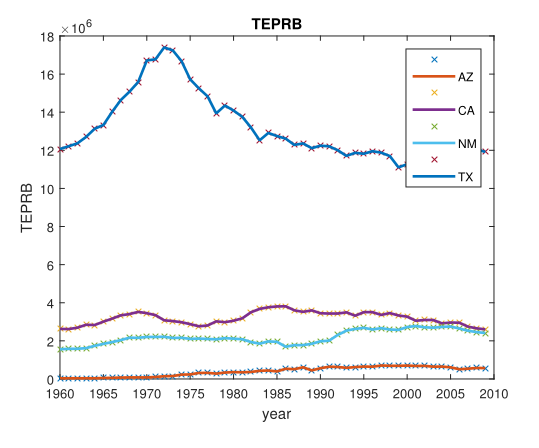
\includegraphics[width=6cm,height=6cm]{a1.png}
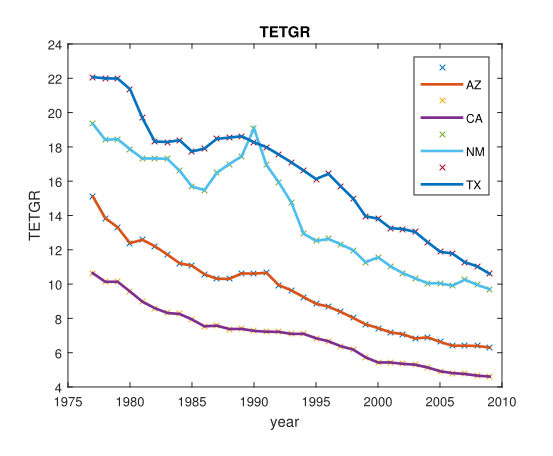
\includegraphics[width=6cm,height=6cm]{a2.png}

From these graphes, we can see:\ \ 1.TX had the largest figures of TEPRB, and AZ had the smallest figures of TETRG.\ 2.The four lines of TETGR did not change a lot except for that of TX.\ 3.The TEPRB of TX peaked in 1990.\ 4.TX had the largest figures of TETGR, and CA had the smallest figures of TETGR.\ 5.The four lines of TETGR generally declined from 1977 to 2009.

To conclude,

1.The total energy production of TX was the largest, and that of AZ was the smallest.CA and NM was moderate.

2.The total energy production did not change a lot in four states except TX,whose total energy production varied shapely around 1990.

3.The energy efficiency of CA was the highest, and that of TX was the lowest.AZ and NM was moderate.

4.The energy efficiency of each state rose up.



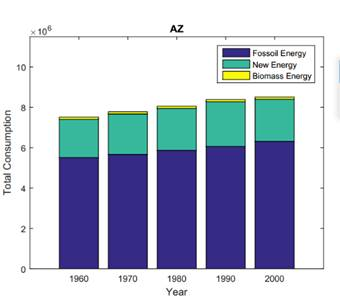
\includegraphics[width=5cm,height=5cm]{AZ.jpg}
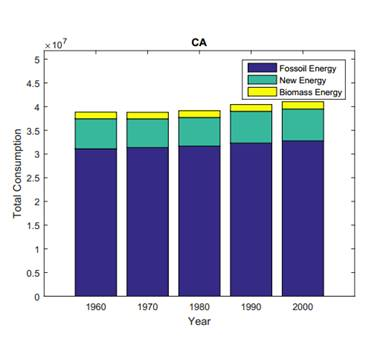
\includegraphics[width=5cm,height=5cm]{CA.jpg}

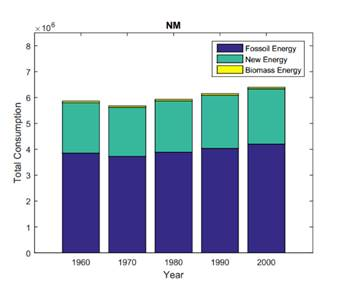
\includegraphics[width=5cm,height=5cm]{NM.jpg}
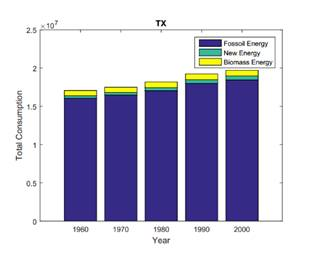
\includegraphics[width=5cm,height=5cm]{TX.jpg}

The four bar graphs above show the total consumption and the proportion of it of three kinds of energy in four states in nearly 50years.

From the four bar charts we can see:\ \ 1.The proportion of total energy consumption(for each state): fossil energy consumption $>$new energy and biomass energy consumption.\ \ 2.The proportion of new energy consumption of total consumption: NA$>$ AZ$>$CA$>$TX.\ 3.The proportion of biomass energy consumption of total consumption: CA, TX$>$ AZ $>$NM.  \ 4.The proportion of fossil energy consumption of total consumption: TX$>$CA$>$AZ$>$NM.


\subsection{Part \uppercase\expandafter{\romannumeral1}  B}

we use the linear regression to get the straight line of regression.

\begin{align*}
x_{A}&= 22753.846t-44372492.94& \\
y_{A} &= 9669.525t-18972804&\\
x_{C}&= 50939.856t-95852654.47& \\
y_{C} &= 18225.574t-35388698&\\
x_{N}&= 9350.545t-17924105.22&\\
y_{N} &= 327.076t-638877.005&\\
x_{T}&= 146324.518t-2.817\cdot 10^{8}& \\
y_{T} &= 13796.265t-27134846.62&\\
\end{align*}

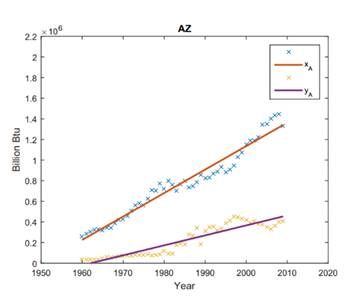
\includegraphics[width=7cm,height=7cm]{b1.jpg}
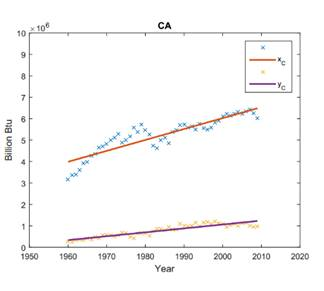
\includegraphics[width=7cm,height=7cm]{b2.jpg}

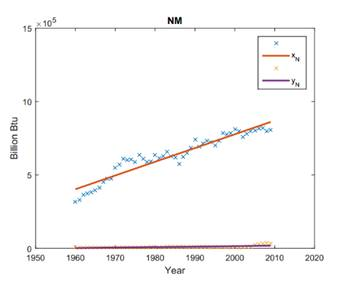
\includegraphics[width=7cm,height=7cm]{b3.jpg}
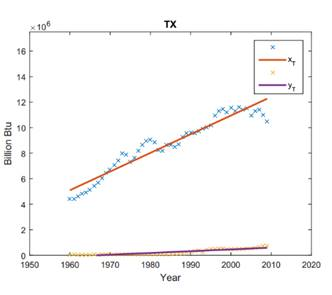
\includegraphics[width=7cm,height=7cm]{b4.jpg}

We analyzed the four graphs, concluding the similarities and differences as follows:

Similarities:

1.The coefficient of $t$ is positive in each graph, suggesting that both new energy and traditional energy consumption of each state increased from 1960 to 2009.

2.The coefficient of traditional energy is larger than that of new energy in each graph, representing the traditional consumption changing rate was higher than the new energy from 1960 to 2009.

Differences:

1.The variable x of TX and CA is larger than that of NM and AZ . This indicates that TX and CA consumed more traditional energy than the other.

2.The slope of new energy in AZ and CA is higher than that of NM and TX. This indicates that the AZ and CA explore new energy more quickly than the other.

To take a better look at the consumption of each kind of new energy, we gathered the data of EMFDB, GETCB, HYTCB, NUTCB, SOTCB, WYTCB, WWTCB.

these 4 graphs below correspond AZ, CA, NM, TX(from left to right, from top to bottom)

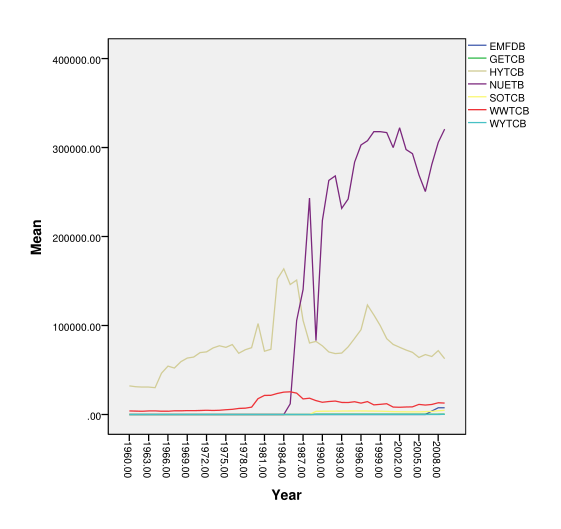
\includegraphics[width=7cm,height=7cm]{b5.png}
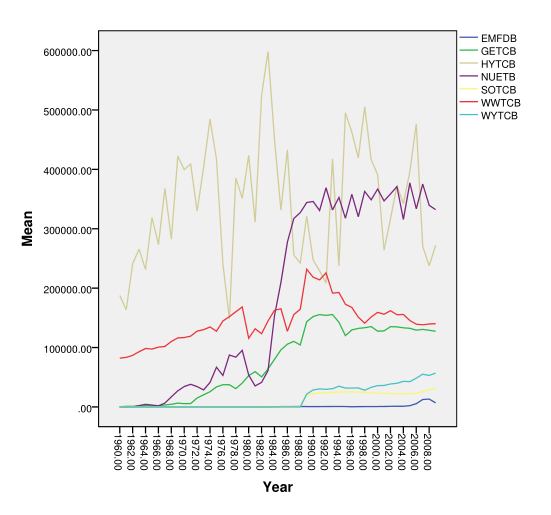
\includegraphics[width=7cm,height=7cm]{b61.png}

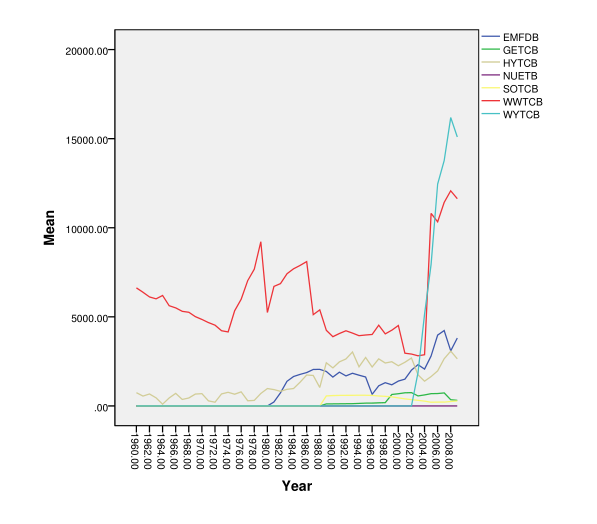
\includegraphics[width=7cm,height=7cm]{b7.png}
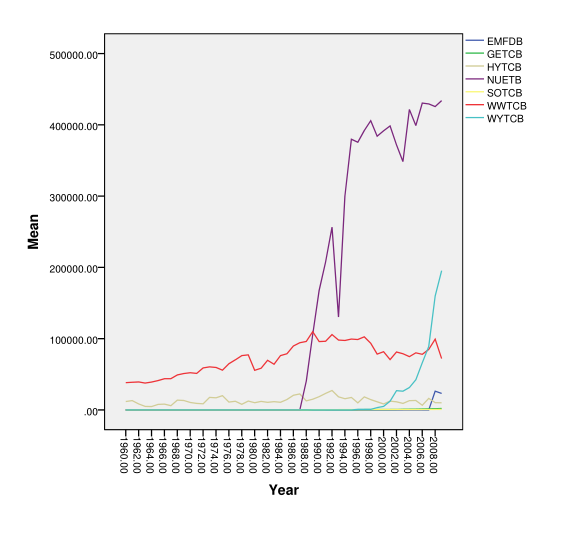
\includegraphics[width=7cm,height=7cm]{b81.png}


After analyzing the four graphs, we found the similarities and differences as follows:

Similarities:

1.The nuclear energy was one of the main energy in AZ, TX and CA. The nuclear energy consumption rose up rapidly from 1985 to 2009.

2.The hydroelectricity energy was one of main energy in AZ and CA from 1960 to 2009.

3.The wood waste energy was one of main energy in TX and NM. from 1960 to 2009.

Differences:

We ranked the population and the GDP of total industry in four states. And we use the GDP of total industry to define its degree of industry development.

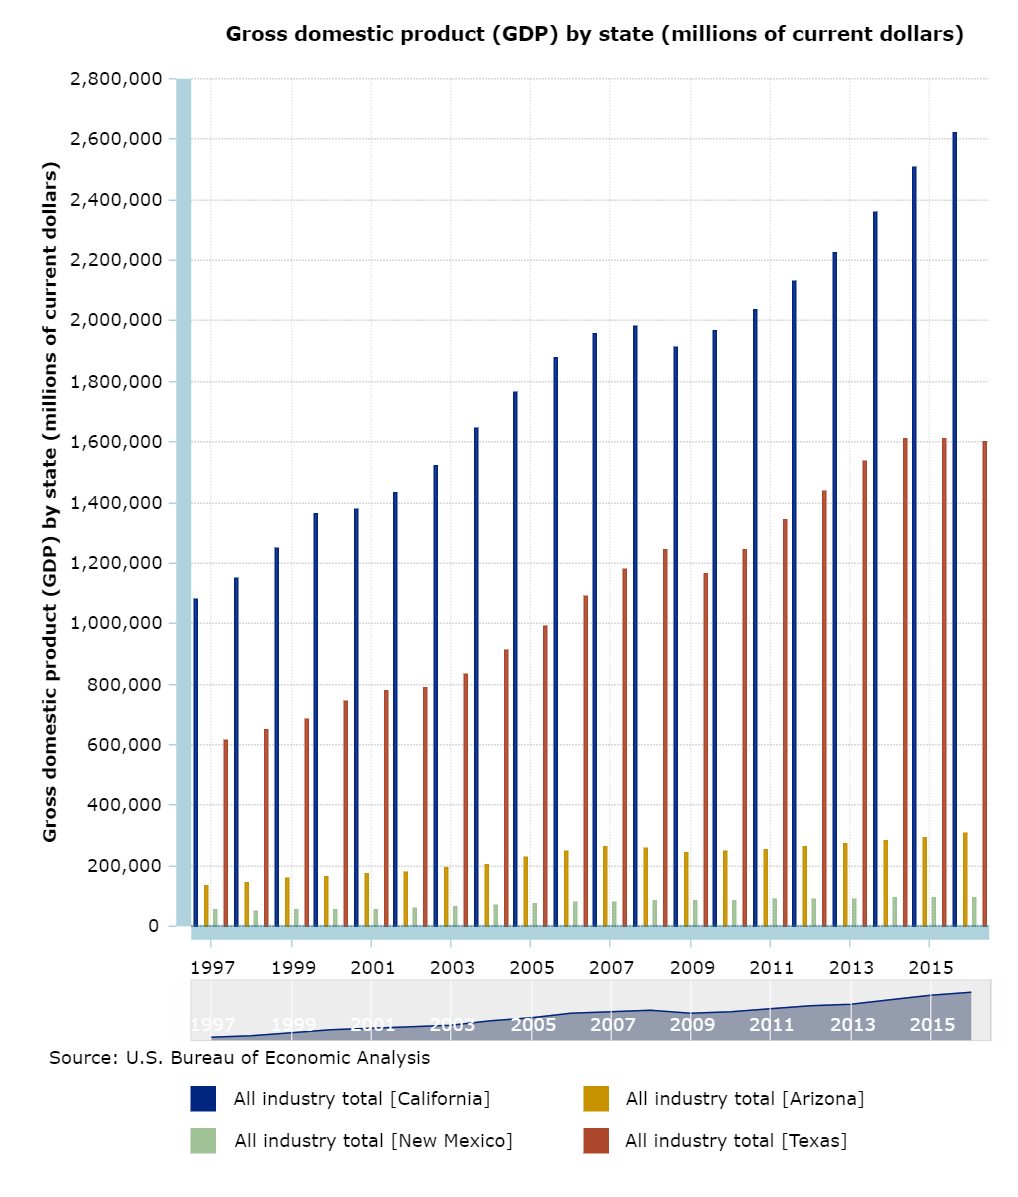
\includegraphics[width=7cm,height=7cm]{b13.jpg}
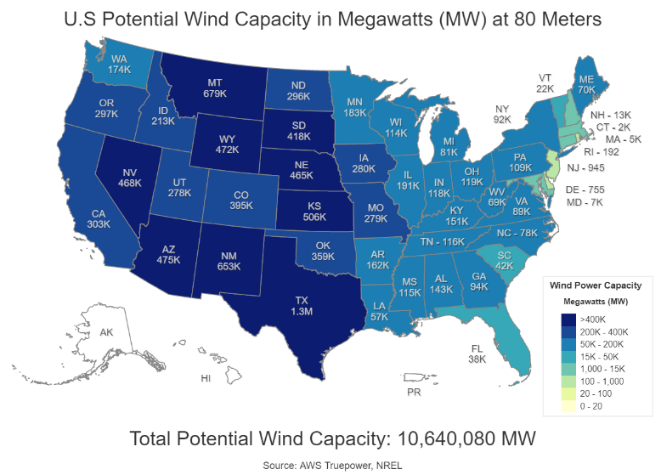
\includegraphics[width=7cm,height=7cm]{b12.png}

In four states, between 1960 and 2009

1.Water resources:
We found that AZ, TX and CA use more nuclear energy, but NM didn't choose nuclear as their primary energy.
 The reason why the major new energy consumption of AZ, TX and CA was nuclear energy is they were near water and had enough cooling resources.

2.Population:
We can see from the pictures that CM has a larger population than others states.
So, it was convincible that CM has the largest energy consumption.

3.Wind potential:
We can know from the pictures that the TX and NM are abundant in wind potential.
So, we thought this is the reason why their wind energy consumptions are large.






\subsection{Part \uppercase\expandafter{\romannumeral1}  C}



\subsubsection{Problem analysis}

To find some indicators to value the extent of cleaner and renewable, we considered whether the energy is renewable and chose carbon dioxide emissions and the amount of pollutants they produced when they burned as the indexes, and evaluated the standard of cleaner renewable regard to energy consumption in the four states.

The principle is: Calculate the emissions of carbon dioxide, sulfur dioxide, nitrogen oxides, and PM2.5 in each state. The more carbon dioxide, sulfur dioxide, nitrogen oxides, and PM2.5 emissions, the higher degree of not cleaner . The longer renew period, the higher degree of renewable. Then, use TOPSIS method to work out the sum of the five aspects as the total score. Finally, comparing these scores to find out which is the best.

\subsubsection{Model hypothesis}

1. Defining the emissions of $\mathrm{CO_{2}}$, $\mathrm{SO_{2}}$, $\mathrm{NO}_{x}$, $\mathrm{PM_{2.5}}$ as the indexes of measuring the standard
of cleaner.

2. To avoid double-counting, we only considered the environment impact from the
consumption of primary energy.

3. The environment of every states will be influenced merely by the energy they consumed in
the states, and won��t be impacted by their neighbors.

4. Geothermal, hydroelectricity, nuclear, solar and wind energy are all clean, which means no sulfur dioxide, nitrogen oxides and PM2.5 emissions when using and ignoring the carbon dioxide emissions from geothermal energy.

5. Because it's easy to remove the sulfur impurities from the natural gas in the process of development and the gas can be sufficient burning, we believed that the natural gas is free of sulfur dioxide and PM2.5.

6. Because the molecular composition of Wood and Waste is close to the biomass, we believed that their combustion has the same effect on the environment.

7. Because the renew period of oil, natural gas and nuclear energy is much longer than that of biomass, solar energy and wind energy. Therefore, we only use 0 and 1 to represent the level of renewable.

8. Suppose that the five aspects mentioned above share the same weight in the evaluation process.

\subsubsection{TOPSIS method}

Notations and description:

\begin{table}[h!]\centering\scriptsize
\begin{tabular}{|c|c|c|c| }
\hline
 \textbf{Notation}&\textbf{Description}&\textbf{Notation}&\textbf{Description}\\
 \hline
$C$&total emission of $\mathrm{CO}_{2}$&$S$&total emission of $\mathrm{SO}_{2}$\\
\hline
$N$&total emission of $\mathrm{NO}_{x}$&$P$&total emission of $\mathrm{PM}_{2.5}$\\
\hline
$R$&total renewable index&$C'$&$C$/GDP\\
\hline
$S'$&$S$/GDP&$N'$&$N$/GDP\\
\hline
$P'$&$P$/GDP&$R'$&$R$/GDP\\
\hline
$c$&$C'$after normalization&$s$&$S'$after normalization\\
\hline
$n$&$N'$after normalization&$p$&$P'$after normalization\\
\hline
$r$&$R'$after normalization&$D^{+}$&distance from the Best Alternative\\
\hline
$D^{-}$&distance from the Worst Alternative&$e$&final index to evaluate\\
\hline
\end{tabular}
\end{table}

We evaluate these 5 indexes, $C,S,N,P,R$.Considering different economy in different state, we use $C',S',N',P',R'$ to offset the effect because of different GDP.

Then, after normalization, (such as $c_{A}=C'_{A}/\sqrt{C'^{2}_{A}+C'^{2}_{C}+C'^{2}_{N}+C'^{2}_{T}}$),

Thus, we get the 5 values after normalization for each state.

$(c_{A},s_{A},n_{A},p_{A},r_{A})$,$(c_{C},s_{C},n_{C},p_{C},r_{C})$,$(c_{N},s_{N},n_{N},p_{N},r_{N})$ and $(c_{T},s_{T},n_{T},p_{T},r_{T})$.

According to our assumptions, the higher these 5 values, the worse in the renewable and cleaner energy use.

So, the Best Alternative is (0,0,0,0,0),and the Worst Alternative is (1,1,1,1,1).
and $$D^{+}=\sqrt{c^{2}+s^{2}+n^{2}+p^{2}+r^{2}}$$

$$D^{-}=\sqrt{(c-1)^{2}+(s-1)^{2}+(n-1)^{2}+(p-1)^{2}+(r-1)^{2}}$$

For one solution, the nearer to the Best Alternative and the farther from the Worst Alternative, the better it is.

so we use $$e=\frac{D^{-}}{D^{+}+D^{-}}$$ to evaluate whether one solution is best.

\subsubsection{Model solving}

We searched the data about emissions of each kind of energy, and use the renewable index we assumed.

\begin{table}[h!]\centering\scriptsize
\begin{tabular}{|c|c|c|c|c|c| }
\hline
& $\mathrm{CO_{2}}$& $\mathrm{SO_{2}}$& $\mathrm{NO}_{x}$& $\mathrm{PM_{2.5}}$&renewable\\
\hline
coal	&888	&10	&4.8	&2.2	&1\\
\hline
petroleum	&733	&6	&17.2	&2	&1\\
\hline
biomass	&45&	1.8	&3	&12.8	&1\\
\hline
geothermal&	0	&0	&0	&0	&0\\
\hline
hydroelectricity&	26	&0	&0&0	&0\\
\hline
nuclear	&29&	0	&0	&0&	1\\
\hline
solar	&85&	0	&0	&0&0\\
\hline
wind	&26&	0	&0	&0	&0\\
\hline
wood and waste	&45	&1.8	&3	&12.8&	0\\
\hline
natural gas	&499	&0&	3.2&	0&	1\\

\hline
\end{tabular}
\end{table}

Then, use Excel calculate every variable.

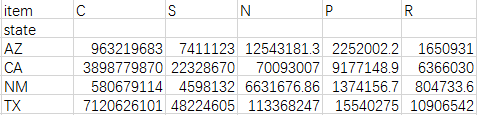
\includegraphics[width=7cm,height=3cm]{c2.png}
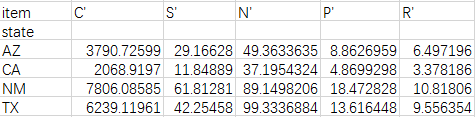
\includegraphics[width=7cm,height=3cm]{c3.png}

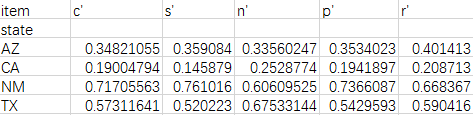
\includegraphics[width=7cm,height=3cm]{c4.png}
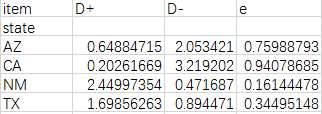
\includegraphics[width=7cm,height=3cm]{c5.png}

As a conclusion, the "best" usage of cleaner and renewable energy is CA.

\subsection{Part \uppercase\expandafter{\romannumeral1}  D}

\subsubsection{Problem analysis}

 The requirements of the subject is to predict the data from 2025 to 2050 on condition that the current policy won��t be changed. Then, considering that from 1960 to 2009, there might be some changes and adjustments in policy, we must narrow the time range to make sure the policy is relatively stable. Therefore, we chose a period of time between 1990 to 2009 as a sample, and used them to predict the data we need.


We calculated the x and y energy of all States respectively, then, we used linear regression to analyze

First of all, we should do significance test.



\begin{table}[!h]\centering
\begin{tabular}{|c|c|c|c|c| }
\hline
Sig&	AZ	&CA&	NM	&TX\\
\hline
$x$	&0.000 &	0.000 &	0.000 &	0.001\\
\hline
$y$	&0.262 &	0.478 &	0.000 	&0.000\\

\hline
\end{tabular}
\end{table}

The results show that the y energy of AZ and x energy of AC cannot be predicted with the linear model under the F-test, so it��s necessary to find some non-linear models. But others can be predicted by linear models. The results of SPSS are as follows:
\begin{align*}
x_{A}&=36111.255t-7109258761&\\
x_{C}&=46254.607t-86544016.79&\\
x_{N}&=5829.083t-10886871.22&\\
y_{N}&=1316.295t-2617330.899&\\
x_{T}&=82157.476t-153500000&\\
y_{T}&=18523.000t-36544604.29&
\end{align*}


As for the $y$ energy of AZ and $y$ energy of CA, we made up the images according to the data.

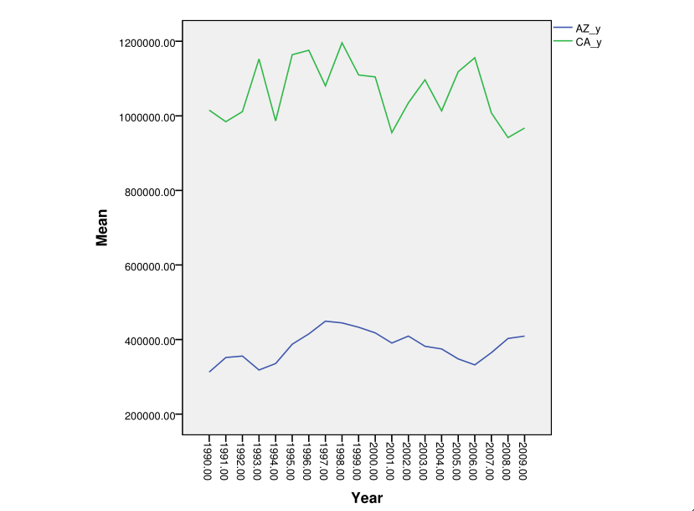
\includegraphics[width=13cm,height=9cm]{d1.png}

The analysis of the image shows that the two images fluctuate drastically but with period regularity. In order to fit the data, we use the polynomial curve fitting.

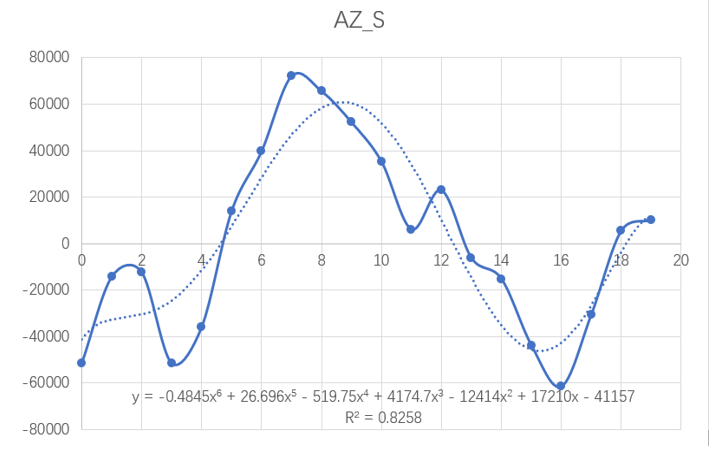
\includegraphics[width=13cm,height=9cm]{d2.png}

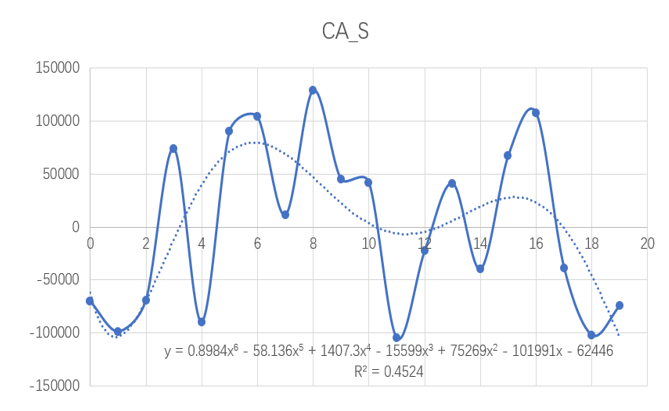
\includegraphics[width=13cm,height=9cm]{d3.png}

Regard the function above as a periodic function, and the period of it is 20, then, calculate the predicted value from 2025 to 2050.

\begin{table}[!h]\centering
\begin{tabular}{|c|c|c|c|c|c| }
\hline
&$y_{A}$&	$y_{C}$&&$y_{A}$&	$y_{C}$\\
\hline
2025&	435809.9&	1409925.996&2038&	449210.5&	1321402.538\\
\hline
2026&	458566.4&	1407776.73&2039&	466507.1&	1295824.272\\
\hline
2027&	478780&	1405536.464&2040&	414660.7&	1378286.006\\
\hline
2028&	492241.6&	1403153.198&2041&	424964.2&	1376142.74\\
\hline
2029&	496089.2&	1400543.932&2042&	428982.8&	1374074.474\\
\hline
2030&	489394.8&	1397580.666&2043&	436795.4&	1372029.208\\
\hline
2031&	473399.4&	1394083.4&2044&	451660&	1369971.942\\
\hline
2032&	451407&	1389801.134&2045&	472341.6&	1367880.676\\
\hline
2033&	428323.5&	1384402.868&2046&	495098.2&	1365731.41\\
\hline
2034&	409847.1&	1377458.602&2047&	515311.8&	1363491.144\\
\hline
2035&	401313.7&	1368427.336&2048&	528773.4&	1361107.878\\
\hline
2036&	406189.3&	1356642.07&2049&	532620.9&	1358498.612\\
\hline
2037&	424216.9&	1341291.804&2050&	525926.5&	1355535.346\\
\hline
\end{tabular}
\end{table}


According to the linear regression and polynomial model, we got the predictions from 2025 to 2050.

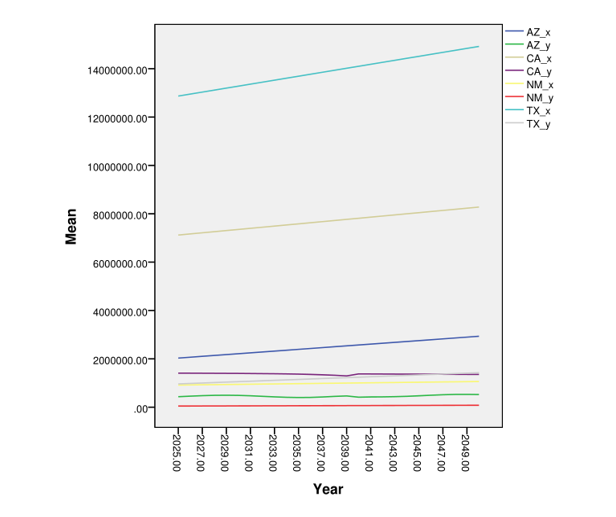
\includegraphics[width=13cm,height=9cm]{d4.png}

\section{Part \uppercase\expandafter{\romannumeral2}}

\subsection{Part \uppercase\expandafter{\romannumeral2}  A}

According to the analysis above, we can make the target of energy consumption. Considering that the four states should be more environmentally friendly, they'd better reduce fossil fuel combustion and increase the consumption of cleaner renewable as far as possible. Therefore, in the prediction internals we get already, when $x$ and $y$ approaching the $x_{2}$ and $y_{1}$ respectively, we can get the most satisfying condition. Thus, we choose the values of $x_{2}$ as the targets for renewable energy consumption and $y_{1}$ as the targets for fossil fuel consumption.

\subsection{Part \uppercase\expandafter{\romannumeral2}  B}

On the aspect of population, geography and industry; emissions of pollutants and the price of energies, we put forward three suggestions.

\subsubsection{Action 1}
First, we assume that energy consumption is equal to the energy production.

According to the conclusion of task B of part I, we have suggestions as follows:

1. Since it was a traditional way for TX, CA and AZ of consuming nuclear energy and in these states nuclear infrastructure facilities were well-built, it could make it easy for these three states to continue following its traditional pattern (using nuclear power the most).

2. Another widely used new energy in CA and AZ was hydroelectricity. CA and AZ were rich in hydroelectricity. As a result of it, we suggest the two states also develop hydroelectricity.

3. The major used new energy in NM was wood waste and wind energy. NM was abundant in wind potential. In view of it, we suggested NM develop wind energy.

\subsubsection{Action 2}

Based on the normalized data obtained from problem C in Part 1, we can find that the largest emissions of NM and AZ was $\mathrm{SO}_{2}$ and the largest emissions of CA and TX was $\mathrm{NO}_{x}$.

1.From the maps that described the major sources of emissions, we found that $\mathrm{SO}_{2}$ emissions primarily from burling coal and the nitrogen oxides emissions mainly from burling oil. So, we recommended AZ and NM to reduce the coal consumption and CA and TX to reduce the oil consumption.

2.According to the data in task C and the following tables, we can find more precise conclusions.

\begin{table}[h!]\centering\scriptsize
\begin{tabular}{|c|c|c|c|c|c| }
\hline
& $\mathrm{CO_{2}}$& $\mathrm{SO_{2}}$& $\mathrm{NO}_{x}$& $\mathrm{PM_{2.5}}$&renewable\\
\hline
coal	&888	&10	&4.8	&2.2	&1\\
\hline
petroleum	&733	&6	&17.2	&2	&1\\
\hline
biomass	&45&	1.8	&3	&12.8	&1\\
\hline
geothermal&	0	&0	&0	&0	&0\\
\hline
hydroelectricity&	26	&0	&0&0	&0\\
\hline
nuclear	&29&	0	&0	&0&	1\\
\hline
solar	&85&	0	&0	&0&0\\
\hline
wind	&26&	0	&0	&0	&0\\
\hline
wood and waste	&45	&1.8	&3	&12.8&	0\\
\hline
natural gas	&499	&0&	3.2&	0&	1\\

\hline
\end{tabular}
\end{table}

We use the data in tables above and the data provided in excel to calculate the source of $\mathrm{SO}_{2}$ emissions from AZ and NM. Take AZ as an example: We multiplied one kind of energy consumed by AZ with $\mathrm{SO}_{2}$ emissions produced by burning this energy per unit. Then we obtained the total $\mathrm{SO}_{2}$ emissions from this type of energy. Finally, we worked out the main causes of emissions. Similarly, we calculated the data related to $\mathrm{SO}_{2}$ in NM, as well as the data related to $\mathrm{NO}_{x}$ in CA and TX.

Then, we deleted the zero terms, and create two tables:

1. (the emission of SO2 from different energy)

\begin{table}[!h]\centering
\begin{tabular}{|c|c|c|c|c| }
\hline
Item&	CLTCB&	PATCB&	EMFDB&	WWTCB\\
\hline
AZ&	4132600&	3241600	&13700&	23200\\
\hline
NM&	3061600	&1508700&	6900&	20900\\

\hline
\end{tabular}
\end{table}
From this chart, we can see that AZ and NM should decline the use of CLTCB and PATCB.


2.(the emission of $\mathrm{NO}_{x}$ from different energy)

\begin{table}[!h]\centering
\begin{tabular}{|c|c|c|c|c| c|}
\hline
	&CLTCB	&PATCB	&EMFDB&	WWTCB&	NGTCB\\
\hline
CA	&252000	&61748000&	21000	&420000	&7652000\\
\hline
TX	&7190000	&94813000	&70000	&216000	&11079000\\
\hline
\end{tabular}
\end{table}

From the chart, we can see that CA and TX should decline the use of PATCB and NGTCB.




\subsubsection{Action 3}

In order to make the state which has the worst environment and less GDP to achieve the goals we made above, it is critical to consider the energy changing among four states. Firstly, we make some hypothesis:

1. With the help of cables and pipelines, the transportation cost regard to electricity and gas among these states can be ignored.

2. The price of electricity in different states are the same and there is no difference on the export prices of electricity between any two states.

3. The electricity they purchased from other states influenced their environment little.

We take coal, petroleum, natural gas and wood and waste into consideration, and suppose the price of electricity is the same as 2009.


\begin{table}[!h]\centering
\begin{tabular}{|c|c|c|c|c| c|}
\hline
	&CLTCD&	NGTCD&	PATCD&	WWTCD&	ESTCD\\
\hline
AZ&	1.82553&	6.38089&	17.18042&	7.83257&	28.00765\\
\hline
CA	&2.66232&	6.37809&	17.71125&	3.9352&	38.90736\\
\hline
NM&	1.9015&	5.95016&	17.64435&	9.83465&	23.96256\\
\hline
TX&	1.89361&	4.65043&	15.07646&	3.62018&	29.20894\\

\hline
\end{tabular}
\end{table}

	CLTCD	NGTCD	PATCD	WWTCD	ESTCD
AZ	1.82553	6.38089	17.18042	7.83257	28.00765
CA	2.66232	6.37809	17.71125	3.9352	38.90736
NM	1.9015	5.95016	17.64435	9.83465	23.96256
TX	1.89361	4.65043	15.07646	3.62018	29.20894

According to the data, we have some suggestions:

1. AZ, NM and CA can purchase natural gas from TX to get cheaper resources.

2. CA and TX can sell wood and waste to other states if the sum of transportation cost and the export price of CA and TX is lower than the price in other states.

3. NM should better reduce the consume of wood and waste and natural gas which is relatively cheap can be a substitution.

4. It��s a greater choice for CA to buy cheaper electricity from other states and decrease the consumption generated in the state.


\section{Part \uppercase\expandafter{\romannumeral3}}

MEMO

To: The group of Governors

From: Our team

Date: 13 February

Subject: Analysis and prediction of energy usage in CA, AZ, NM and TX
\newline
\newline
\indent Mr./ Mrs. Governor, we are writing to report you our key findings in these four days of analysis and prediction of energy usage in four states. We divided the findings into two parts.

In the first part, we concluded state profiles as of 2009: first of all, the total energy consumed per dollar of GDP generally declined in each state, indicating that the increase of energy efficiency of four states. Next, the total energy consumed per dollar of GDP of CA, NM and AZ has no significant changes.
Besides, the traditional energy and new energy consumption of each state rose up. TX was the state consumed the largest of traditional energy, oppositely was NM. Then, CA, TX and NM mainly consumed nuclear energy; while NM mainly consumed waste wood energy. Finally, CA appeared to have the ��best�� profile for use of cleaner, renewable energy in 2009.

In the second part, we predicted the ��best�� profile and set goals in the absence of any policy changes by each governor��s office from 2025 to 2050. We also predicted new energy and traditional energy consumption of each state with the 95\% possibility in a range from 2025 to 2050.


\section{\leftline{Strengths and weaknesses}}
\subsection{Merits}

  1.To analyze the data of 4 states from 1960 to 2009, we use the linear regression to find the quantity and the tendency with the time. All the linear model has passed significance test(significance level $\alpha=0.01$), which means our model is accurate and reasonable.

  2.We searched 5 indexes and their data, and next used the TOPSIS method to evaluate which is the ��best�� in cleaner and renewable energy usage. It could make our result objective and rational.

 3.In the prediction, we predicted both the most likely quantity and the prediction intervals(significance level $\alpha=0.05$). Consequently, the governs may attain more data they want.

\subsection{Defects}
 1.In the TOPSIS method, we failed to confirm the weight of 5 indexes because of the lack of data.


  2.In the prediction model, we used the polynomial to fit the data which cannot be fit by linear model. We did not test other curves to achieve the best results.

\section{\leftline{References}}

1. World Energy Outlook Special Report (2016). [online]. International Energy Agency (ING). Available from: January 13, 2018

at: https://www.iea.org/publications/freepublications/publication/weo-2016-special-report-energy-and-air-pollution.html


2. WNA Report Comparison of Lifecycle Greenhouse Gas Emissions of Various Electricity Generation Sources. [online]. World Nuclear Association (WNA). Available from: January 13, 2018

at: http://www.world-nuclear.org/uploadedFiles/org/WNA/Publications/Working-Group-Reports/comparison-of-lifecycle.pdf


3. The information about U.S. Potential Wind Power Capacity and Generation.

https://windexchange.energy.gov/maps-data/321


4. The information about U.S. industry at https://www.bea.gov/iTable/index-industry-gdpIndy.cfm


5.The information about advantages of interstate energy corporation

at  http://www.gsgp.org/media/1313/understanding-interstate-compacts-csgncic.pdf

6.The information about Southern States Energy Board (SSEB)

https://en.wikipedia.org/wiki/Southern-States-Energy-Board







\end{document}
